\section{Tutorial Using Reverse-Slip Without Gravity Benchmark}

\subsection{Overview}

In this tutorial, we will walk through the steps necessary to
construct, run, and view the results of a benchmark problem involving
reverse slip on a dipping fault. This problem examines the
viscoelastic (Maxwell) relaxation of stress from a single, finite,
reverse-slip earthquake in 3-D without body forces.


\subsection{Problem Description}

The model domain is a cube with edges 24 km long (0 km $\leq$ x $\leq$
24 km; 0 km $\leq$ y $\leq$ 24 km; -24 km $\leq$ z $\leq$ 0) and
is composed of two materials. One material occupies the top-half of
the domain, -12 km $\leq$ z $\leq$ 0 km, while the other occupies
the lower half, -24 km $\leq$ z $<$ 12 km. Both materials are Poisson
solids with Lame's constants ($\mu$ and $\lambda$) equal to 30 GPa and
Maxwell viscoelastic properties. The top layer has a viscosity of
$10^25$ Pa-s (and is essentially elastic) while the bottom layer has a
viscosity of $10^18$ Pa-s.

The reverse fault dips at an angle of 45 degrees. The top of the fault
sits at x = 4 km with the bottom of the fault at x = 20 km. The fault
surface is confined to the region 0 km $\leq$ y $\leq$ 16 km and -16
km $\leq$ z $\leq$ 0 km. The slip distribution is 1.0 m of uniform
thrust motion for -12 km $\leq$ z with a linear taper to 0 at z = -16
km.

The plane y=0 is a plane of symmetry, so the y-DOF displacements on
this face are zero. The boundary conditions on the other lateral faces
and bottom of the mesh are the displacements from the analytical
elastic solution. These displacements are held fixed through time.

\begin{figure}
  \begin{center}
    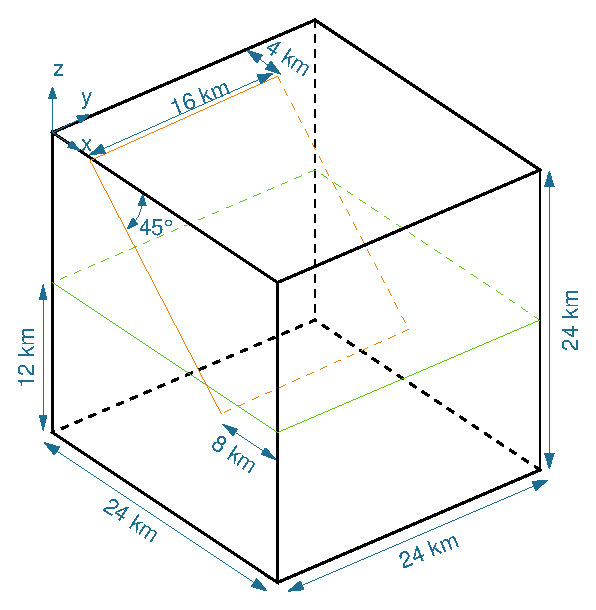
\includegraphics{figs/geometry}
    \caption{Geometry of model domain for reverse-slip benchmark.}
  \end{center}
\end{figure}  

\subsubsection{Workflow}

The complete workflow used to create the input files for this tutorial
is shown in figure~\ref{fig:bmrsnog:workflow}. Because some of the
steps involve commercial software (e.g., Matlab), we will skip those
steps in this tutorial.

\begin{figure}[htbp]
  \begin{center}
    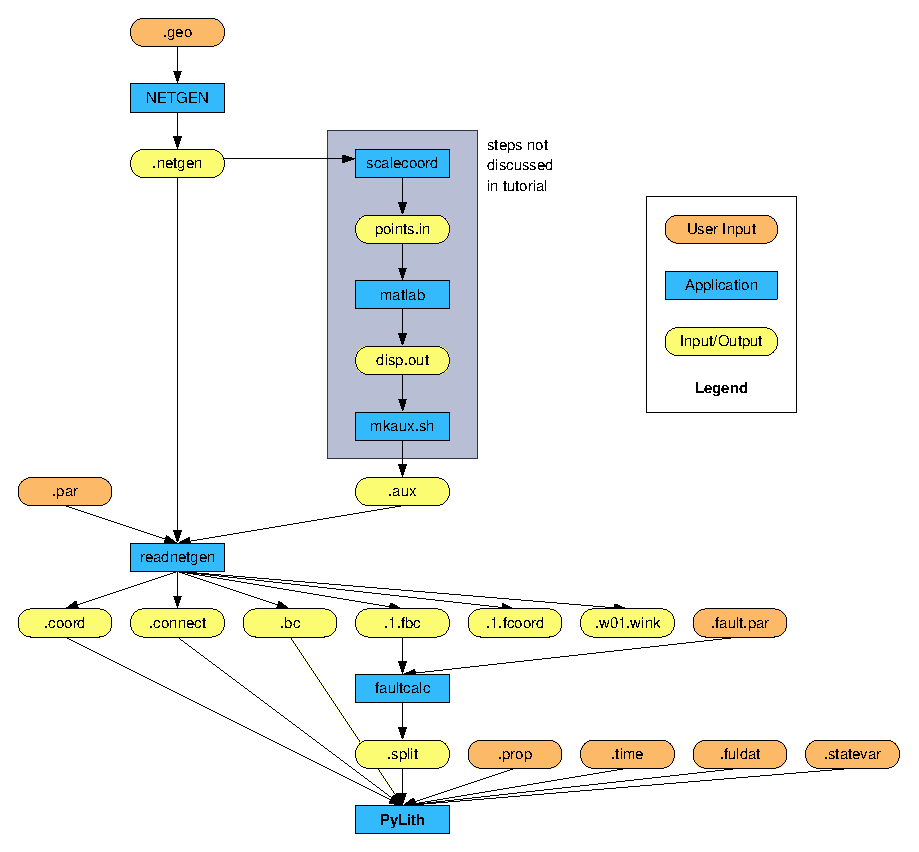
\includegraphics{figs/workflow}
    \caption{Workflow for setting up input files for benchmark with reverse
      slip and no gravity.}
    \label{fig:bmrsnog:workflow}
  \end{center}
\end{figure}

\subsection{Download and unpack}

We will start by downloading the tutorial tarball and unpacking it.

\begin{enumerate}
\item Download the \link{tutorial
    tarball}{http://www.geodynamics.org:8080/cig/Members/willic3/pylithusers/pylith0.8/pylith-0.8\_tutorials.tgz}
  and unpack it in a location of your choosing.

  \begin{screen}
    \shellprompt\userinput{tar -zxvf pylith-0.8\_tutorials.tgz}
  \end{screen}
  
\item Go to the \directory{tutorials/reversenog} directory.
  The \directory{archive} directory contains all of the input and
  output files associated with this tutorial. We will copy input files
  from this directory into the \directory{workarea} directory. At each
  step, you can check to make sure your input and output agree with
  the files in the \directory{archive} directory. These files also
  allow you to start at an intermediate step as described in the next
  section.

  \begin{screen}
    \shellprompt\userinput{cd tutorials/reversenog}
  \end{screen}

\end{enumerate}

\subsection{Tutor}

Copy the \filename{tutor.py} script from the \directory{archive}
directory into the \directory{workarea} directory. 

\begin{tip}
  If you have run this tutorial previously, you may want to run
  \command{tutor.py} in mode "clean" with step "all" to clear out all
  old tutorial files.
\end{tip}

\begin{screen}
\shellprompt\userinput{cd workarea}
\shellprompt\userinput{cp ../archive/tutor.py .}
\shellprompt\userinput{./tutor.py -m clean -s all}
\end{screen}

\subsection{Generate the mesh}

In this step we will generate the finite-element mesh for the
benchmark problem using \application{NETGEN}.

\begin{enumerate}
\item In the \directory{reversenog/workarea} directory, run
  \command{tutor.py} for step "mesh" with mode "retrieve" to fetch the
  geometry file for \application{NETGEN}. You may also want to run
  \command{tutor.py} for this step with mode "clean" to clean out old
  files.

  \begin{screen}
    \shellprompt\userinput{./tutor.py -m retrieve -s mesh}
    \shellprompt\userinput{./tutor.py -m clean -s mesh}
  \end{screen}
  
\item Examine the \filename{bmrsnog.geo} file to see how the geometry
  for the problem is defined. Notice that the different planes have
  been flagged with different boundary condition codes. These will be
  used to associate boundary conditions with surfaces and element
  nodes.
\item Start up \application{NETGEN} by running \command{ng}.

  \begin{screen}
    \shellprompt\userinput{ng}
  \end{screen}
  
\item Select \guimenu{File}\guiselect\guimenuitem{Load Geometry}
  and select \filename{bmrsnog.geo}.
\item Click on \guibutton{Generate Mesh}.
\item Export the mesh to a file named \filename{bmrsnog.netgen},
  making sure the export filetype is "Neutral format".
\item You can now exit \application{NETGEN}.
\end{enumerate}

\subsection{Setup simulation input files}

In this step we will setup the PyLith input files for the mesh and
boundary conditions.

\begin{enumerate}
\item Run \command{tutor.py} for step "setup" with mode "retrieve" to
  fetch files from the archive.

  \begin{screen}
    \shellprompt\userinput{./tutor.py -m retrieve -s setup}
  \end{screen}
  
\item We will use two simple Fortran utilities to generate PyLith
  input files from the \application{NETGEN} output.

  \begin{description}
  \item[\command{readnetgen}] A Fortran program to read
    \application{NETGEN} neutral format and create several of the
    input files needed by PyLith.
  \item[\command{faultcalc}] A Fortran program to compute split node
    displacements using second order polynomials over specified
    regions.
  \end{description}
  
\item Run the \command{readnetgen} utility program to process the
  \application{NETGEN} output file into PyLith compatible input files.
  It will ask for a root filename, enter \filename{bmrsnog}. This
  utilitiy will generate the following files:
  \filename{bmrsnog.w01.wink}, \filename{bmrsnog.coord},
  \filename{bmrsnog.connect}, \filename{bmrsnog.bc},
  \filename{bmrsnog.1.fcoord}, \filename{bmrsnog.1.fbc}.

  \begin{screen}
    \shellprompt\userinput{../../utils/readnetgen}
    \prompt{~Enter root name for all files.  Both input and}\\
    \prompt{~output files will all have this prefix:}\\
    \userinput{bmrsnog}
  \end{screen}
  
\item The boundary conditions on the fault for this benchmark are
  somewhat complex. The utility program \command{faultcalc} creates
  split node boundary conditions over specified regions, using
  functions based on second degree polynomials. The
  \command{readnetgen} program has already produced the main input for
  \command{faultcalc} -- split node definitions in
  \filename{bmrsnog.1.fbc} and nodal coordinates in
  \filename{bmrsnog.coord}. The file \filename{bmrsnog.fault.par}
  contains the polynomial coefficients for this benchmark problem. Run
  \command{faultcalc} to get the \filename{bmrsnog.split} file that
  PyLith needs as input.

  \begin{screen}
    \shellprompt\userinput{../../utils/faultcalc p=bmrsnog.fault.par n=bmrsnog.coord\\
      i=bmrsnog.1.fbc o=bmrsnog.split}
  \end{screen}
  
\item The external boundary conditions for this benchmark are also
  complicated and require computing the displacements for the
  analytical elastic solution at each finite element node on the
  external boundaries. The file specifying these boundary conditions,
  \filename{bmrsnog.bc}, was produced with \command{readnetgen} using
  the \filename{bmrsnog.aux} file (which contains precomputed
  displacements for the external boundaries for the mesh produced from
  the \filename{bmrsnog.geo} geometry).

  \begin{warning}
    If you make any changes to \filename{bmrsnog.geo} or change the
    geometry within \application{NETGEN}, the boundary condition file
    \filename{bmrsnog.bc} will no longer be correct and you will have
    to generate one yourself.  Note that it is also possible that a
    different version of \application{NETGEN} may provide a slightly
    different mesh, which would also be incompatible with the provided
    boundary conditions.
  \end{warning}
\end{enumerate}

\subsection{Run the simulation on one processor}

In this step we will run the simulation on a single processor.

\begin{enumerate}
\item Run \command{tutor.py} for step "run1" with mode "retrieve" to
  fetch some parameter files from the archive.

  \begin{screen}
    \shellprompt\userinput{./tutor.py -m retrieve -s run1}
  \end{screen}
  
\item In \filename{bmrsnog.fuldat}, we have specified that we want
  full output at time steps 10, 50, and 100. We define six materials
  with both elastic and viscoelastic behavior in
  \filename{bmrsnog.prop}. In \filename{bmrsnog.statevar} we choose to
  include total stress, total strain, incremental stress, and
  incremental strain in the output. As defined in
  \filename{bmrsnog.time}, the simulation will have 100 time steps of
  0.1 year each.
\item Run the simulation by executing \userinput{runbm.py -n 1}, where
  the 1 refers to the number of processors.

  \begin{tip}
    All of the input is echoed in the file \filename{bmrsnog.ascii}.
    You can check to make sure your input is digested correctly by
    examining this file. For large problems, this file can be quite
    large. You can suppress creation of this file using the command
    line argument \option{--scanner.asciiOutput=none} flag. On the
    other hand, for debugging purposes in small problems, you may wish
    to output everything, including the computed results, in this file
    using \option{--scanner.asciiOutput=full}.
  \end{tip}
  
  \begin{screen}
    \shellprompt\userinput{./runbm.py -n 1}
  \end{screen}
\end{enumerate}

\subsection{Visualize the single processor run}

Now it is time to visualize the results of the simulation. By default,
PyLith writes simulation output using \link{\application{AVS} UCD
  files}{http://help.avs.com/Express/doc/help/reference/dvmac/UCD\_Form.htm}.
These can be read by several other visualization tools besides
\application{AVS}, e.g., \application{ParaView} and \application{Iris
  Explorer}. We will use the open-source application
\application{ParaView} to visualize the results.
    
\begin{enumerate}
\item If necessary, run \command{tutor.py} for step "viz1" with mode
  "retrieve" to fetch the simulation output from the archive.

  \begin{screen}
    \shellprompt\userinput{./tutor.py -m retrieve -s viz1}
  \end{screen}
  
\item PyLith does not write complete UCD files. So the first step is
  to combine the mesh topology information with the output at a given
  time step into a complete UCD file. For example, use \command{cat}
  to merge the nodal coordinates file
  (\filename{bmrsnog\_1.0.mesh.inp}) and the nodal displacements at
  time step 10 file (\filename{bmrsnog\_1.0.mesh.time.00010.inp}) into
  \filename{bmrsnog\_1.0.mesh.t00010.inp}.

  \begin{screen}
    \shellprompt\userinput{cat bmrsnog\_1.0.mesh.inp bmrsnog\_1.0.mesh.time.00010.inp \ \\
> bmrsnog\_1.0.mesh.t00010.inp}
\end{screen}

\item Start \application{ParaView} by executing \command{paraview}.

  \begin{screen}
    \shellprompt\userinput{paraview}
  \end{screen}
  
\item Load the UCD file that you just created by selecting
  \guimenu{File}\guiselect\guimenuitem{Open Data}. Select the file in
  the dialog box and the click the \guibutton{Open} button. Click the
  \guibutton{Accept} button. You should see a color rendering of the x
  displacements. You can use the mouse to rotate, translate, and zoom.
  Your image should look similar to the one in
  figure~\ref{fig::bmrsnog:xdisp:t10}.
        
  \begin{figure}[htbp]
    \begin{center}
      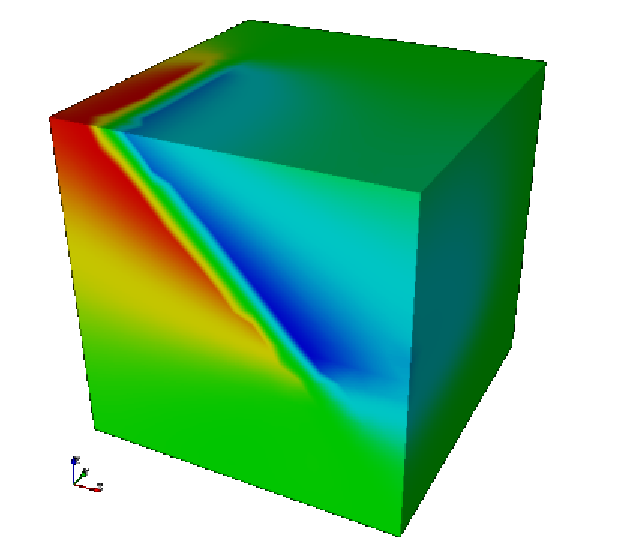
\includegraphics{figs/xdisp_t10}
      \caption{ParaView rendering of displacement in x-direction at
          time step 10 (10 yrs after imposed dislocation) for the
          reverse slip without gravity benchmark.}
      \label{fig:bmrsnog:xdisp:t10}
    \end{center}
  \end{figure}
  
\item In the \guibutton{Display} tab, you can change several options,
  such as including a color bar, coloring a different component,
  interpolating colors, and changing the color map.
\item Let's show the displacements as vectors. Click on the calculator
  icon, and add the three displacement components together. Enter
  "XDispl*iHat+YDispl*jHat+ZDispl*kHat" in the \guimenuitem{Calculator}
  box. Note the variable names are available by clicking on the
  \guibutton{scalars} button and the \guibutton{iHat},
  \guibutton{jHat}, \guibutton{kHat} buttons are on the right side of
  the top row. Click on the \guibutton{Accept} button. To show the
  dataset as vectors, click on the \guibutton{glyph} button (looks
  like several dots) in the toolbar. After clicking the
  \guibutton{Accept} button, you should have a vector plot. You can
  turn on/off other datasets by clicking on the eye icon to the left
  of the dataset name. If you color the surfaces using the
  x-displacements field while also making the displacement vectors
  visible (colored using property), you should see an image similar to
  the one in figure~\ref{fig:bmrsnog:xdisp:vec:t10}.

  \begin{figure}[htbp]
    \begin{center}
      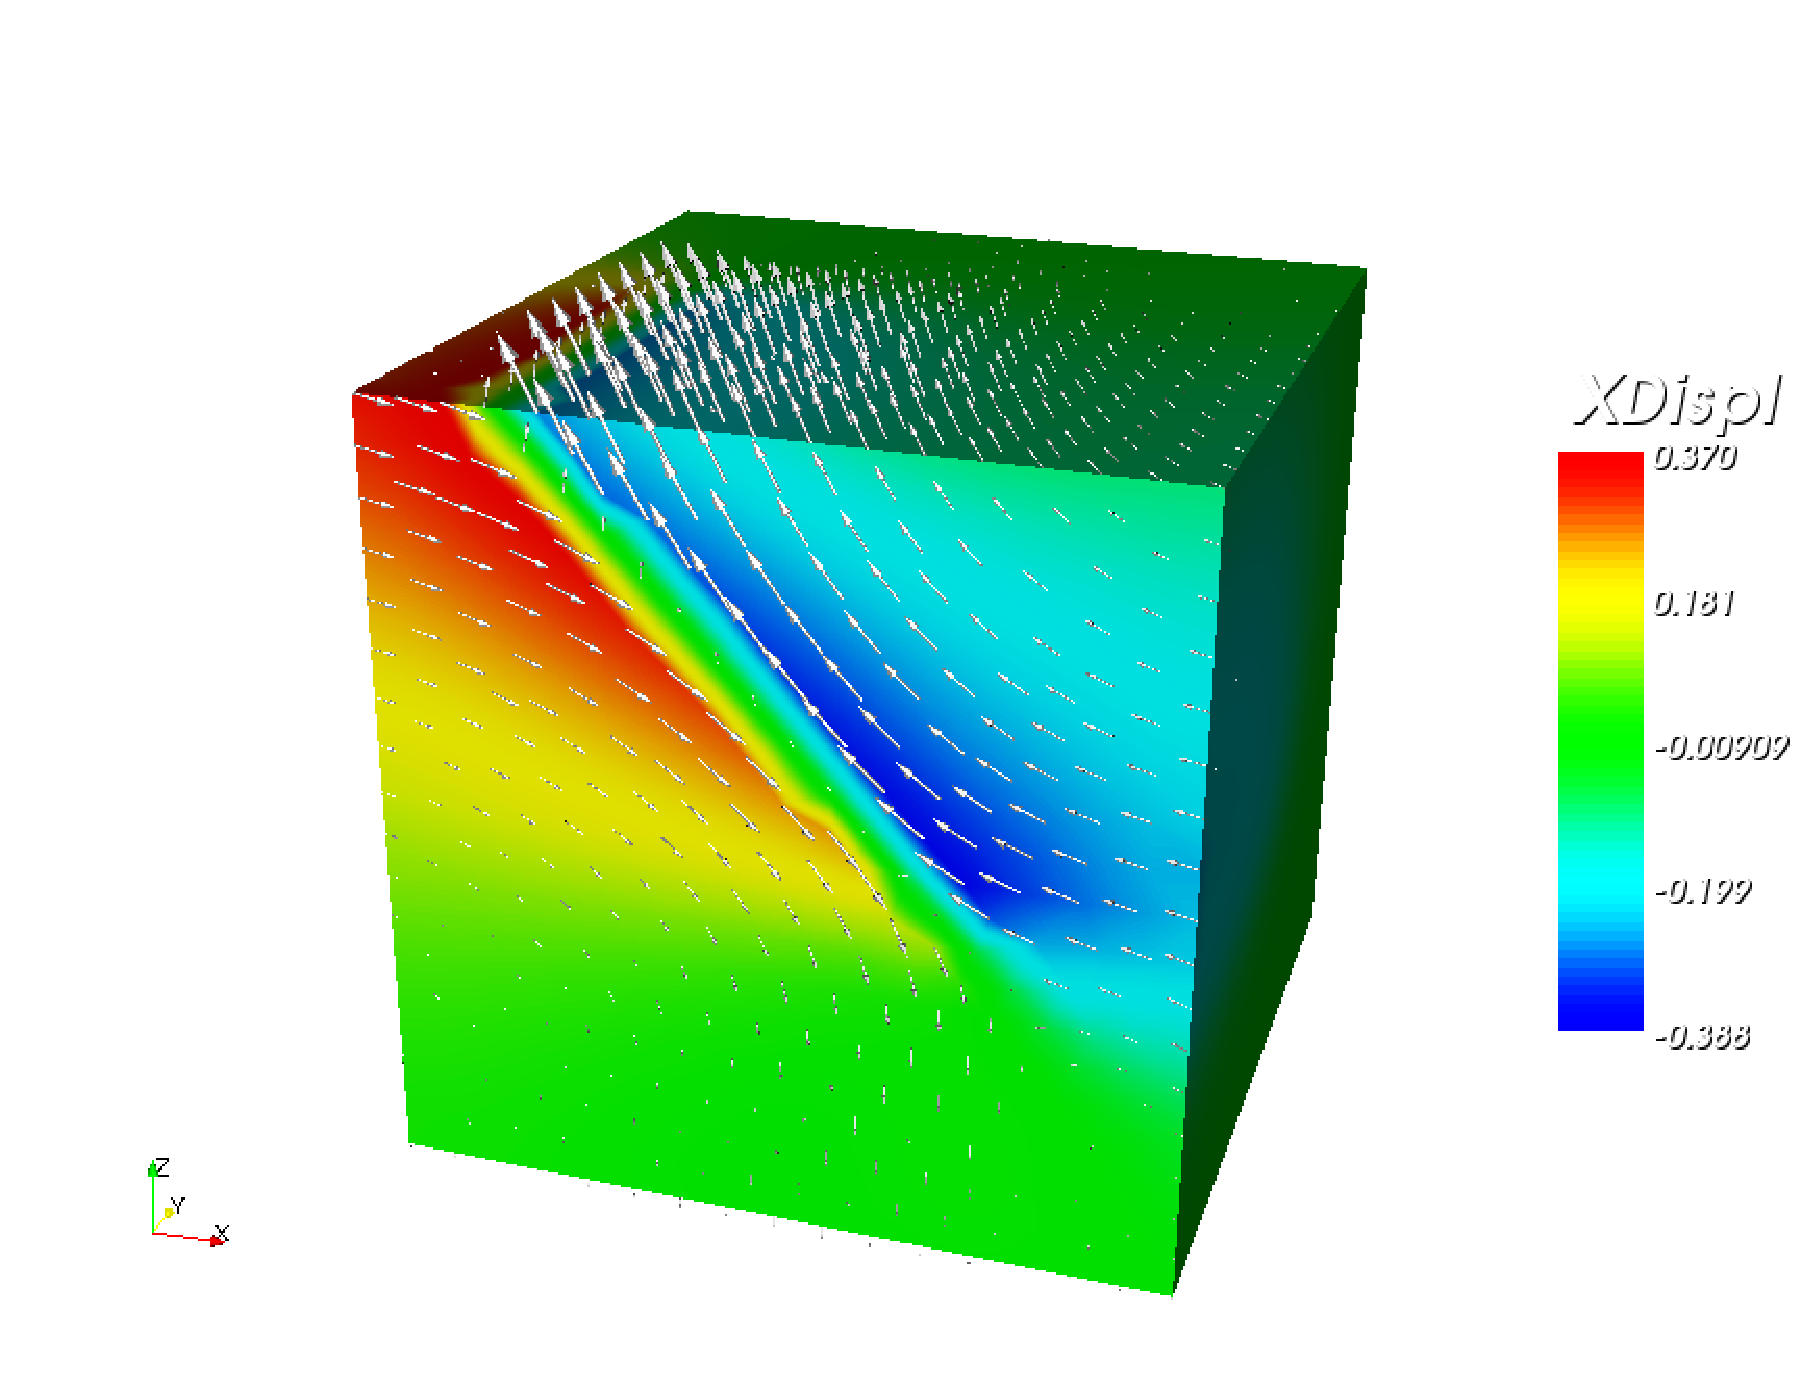
\includegraphics{figs/xdisp_vec_t10}
      \caption{ParaView rendering of displacement in x-direction and
        displacement vectors at time step 10 (10 yrs after imposed
        dislocation) for the reverse slip without gravity
        benchmark.}
      \label{fig:bmrsnog:xdisp:vec:t10}
    \end{center}
  \end{figure}      

\end{enumerate}

\subsection{Run the simulation on two processors}

In this step we will run the simulation on two processors. Even if
your machine only has one processor, a "multprocessor" job will run as
multiple processes on the single processor. In such cases, the job
will run slightly slower than the single processor run, but the two
processes will behave independently as if they are on different
processors.

\begin{enumerate}
\item Run \command{tutor.py} for step "run2" with mode "retrieve" to
  make sure all parameter files are available.

  \begin{screen}
    \shellprompt\userinput{./tutor.py -m retrieve -s run2}
  \end{screen}
  
\item The parameter files are the same as those in the single
  processor run. The \command{runbm} script will automatically take
  care of duplicating these files so that there is one for each
  processor.
\item Run the simulation by executing \command{runbm.py -n 2}, where
  the 2 refers to the number of processors.

  \begin{screen}
    \shellprompt\userinput{./runbm.py -n 2}
  \end{screen}
\end{enumerate}

\subsection{Visualize the two processor run}

PyLith does not currently support parallel output, so each processor
writes its UCD output to a different file. This means that you need to
form complete UCD files for each processor and then load each one into
\application{ParaView}.

\begin{enumerate}
\item If necessary, run \command{tutor.py} for step "viz2" with mode
  "retrieve" to fetch the simulation output from the archive.

  \begin{screen}
    \shellprompt\userinput{./tutor.py -m retrieve -s viz2}
  \end{screen}
  
\item As in the case of the single processor run, the first step is to
  combine the mesh topology information with the output at a given
  time step into a complete UCD file. Because PyLith writes the output
  from each processor into a different file, we must run \command{cat}
  twice to create UCD files for each processor.

  \begin{screen}
    \shellprompt\userinput{cat bmrsnog\_2.0.mesh.inp bmrsnog\_2.0.mesh.time.00010.inp \\
      > bmrsnog\_2.0.mesh.t00010.inp} \\
    \shellprompt\userinput{cat bmrsnog\_2.1.mesh.inp bmrsnog\_2.1.mesh.time.00010.inp \\
      > bmrsnog\_2.1.mesh.t00010.inp}
  \end{screen}

\item Start \application{ParaView} by executing \command{paraview}.

  \begin{screen}
    \shellprompt\userinput{paraview}
  \end{screen}
  
\item Load the UCD files that you just created by selecting
  \guimenu{File}\guiselect\guimenuitem{Open Data}. Select the file in
  the dialog box and the click the \guibutton{Open} button. Click the
  \guibutton{Accept} button. You can now visualize the datasets just
  like you did for the single processor case.
\item You can merge the datasets from the different processors by
  selecting \guimenu{Filter}\guiselect\guimenuitem{Append}. Doing so
  will allow you to operate on the data from all of the processors
  simultaneously instead of having to repeat any processing for every
  processor.
\end{enumerate}
